% o \label{codigo} serve para podermos fazer referencias para algo numerado, 
% como capitulos, tabelas, figuras, etc. 
% Quando colocamos o comando \ref{codigo}. o compilador troca o \ref{codigo}
% pelo numero atribuido ao \label{}
% ex. \label{tabelaLegal}
%   A tabela \ref{tabelaLegal} mostra que...
% vai ser substituido por
%   A tabela 2 mostra que

\chapter{Testes}\label{cap-testes}

Para a avaliação da eficácia do produto final deste trabalho, foi
desenvolvido um questionário, presente no \autoref{apendice:questionario}, 
assim como um roteiro de testes para a aplicação de tal 
questionário. Após a concepção do roteiro de testes, houve 
uma sessão de teste do jogo (\textit{playtesting}) contemplando 
principalmente representantes do público alvo escolhido - crianças 
entre 8 e 12 anos de idade.

As experiências dos jogadores conforme observadas e relatadas foram 
então compiladas em um relatório descrevendo os aspectos positivos e negativos 
do jogo, bem como dificuldades técnicas encontradas.

% ---
\section{Roteiro de Testes}\label{sec-roteiro-testes}
% ---

A concepção do questionário se deu através de duas iterações.

Na primeira iteração, o foco foi no conteúdo das questões. A 
preocupação principal foi o quanto as perguntas ajudariam a 
responder se o jogo era divertido, imersivo e estimulava as 
habilidades do raciocínio lógico. Foram desenvolvidas 13 questões 
com uma escala de 7 pontos (aonde 1 é "Discordo Plenamente" e 7 
é "Concordo Plenamente") e três dissertativas curtas. As questões 
foram divididos em 3 seções: experiência, interface e desafios. 
O primeiro tenta medir a diversão percebida pelo jogador, o segundo 
a imersão e facilidade de interação com o jogo e o terceiro o 
estímulo ao raciocínio lógico.

A segunda iteração ocorreu após a verificação do questionário com 
crianças da faixa etária do público alvo, que foi feita para 
confirmar que o vocabulário utilizado estava adequada e de fácil 
compreensão para o jogador. Visto que foram constatadas 
dificuldades no entendimento em aproximadamente metade das 
questões, o questionário foi reescrito com uma linguagem mais 
simples e novamente verificada com crianças.

Após ter sido verificado com crianças da idade do público alvo, 
foi feita uma validação do questionário com três especialistas 
que são das áreas de educação, jogos, interface com o usuário e 
interação humano-computador.

Para os testes, o seguinte roteiro foi criado:

\begin{alineas}
	\item fornecimento das informações sobre o motivo da pesquisa;
	\item fornecimento de instruções sobre a tarefa a ser realizada;
	\item fornecimento de informações sobre os riscos ao sujeito de pesquisa;
	\item coleta da permissão, concedida pelo guardião legal da criança, para que esta participe do teste.
	\item conectar o \textit{smartphone} do pesquisador que está aplicando o teste ao computador do pesquisador e executar o software do jogo; 
	\item encerrar a sessão de teste após terminar as 4 fases selecionadas, ou após 15 minutos, o que vier antes;
	\item preencher o questionário desta pesquisa.
\end{alineas}

Visto que estamos trabalhando com menores de 18 anos, é necessário 
que o guardião legal da criança conceda permissão para que ela 
participe do teste.	

Esta pesquisa foi aprovada pelo Comitê de Ética em Pesquisa do 
Hospital Universitário da USP (CEP-HU/USP) com parecer 
consubstanciado número 1.114.876 datado de 19/06/2015.

% ---
\section{Playtesting}\label{sec-playtesting}
% ---

A seção de \textit{playtesting} foi realizada durante o Tech Kids Day 
realizado no museu Catavento Cultural no dia 12 de novembro como parte 
da São Paulo Tech Week 2016. 

Uma versão reduzida e simplificada do jogo foi elaborada, contendo uma 
parcela suficientemente representativa do conteúdo do jogo, enquanto 
mantendo o tempo de jogo dentro de um período de 15 minutos ou menos, 
compatível com as condições de teste.

\begin{figure}[h]
	\centering
	\caption{crianças testando o jogo durante a no Tech Kids Day}
	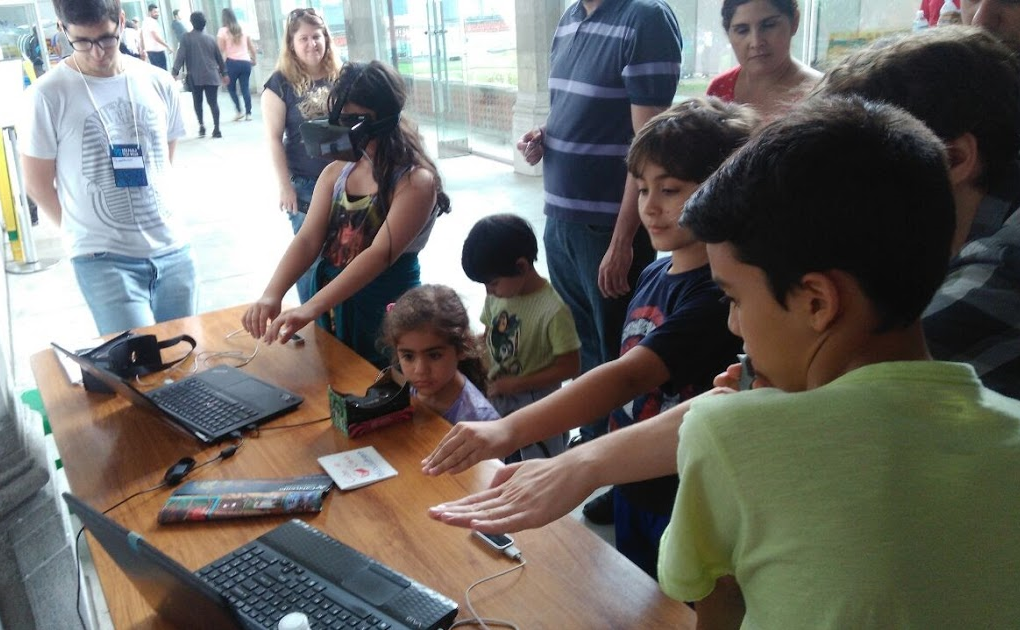
\includegraphics[width=0.5\textwidth]{tech_kids_booth}
	\legend{\fonteAP}
	\label{fig:tech-kids-day}
\end{figure}

Essa versão consiste em um conjunto de 4 fases, dispondo do seguinte conteúdo:

\begin{alineas}
	\item \textbf{fase 1:} introdução ao funcionamento básico do jogo. Apresentação das mecânicas de seleção em área e manipulação da elevação do terreno;
	\item \textbf{fase 2:} introdução de mecânicas de criação e manipulação de corpos d'água;
	\item \textbf{fase 3:} introdução da mecânica de vento e da criação de blocos de areia;
	\item \textbf{fase 4:} combinação de todos os elementos apresentados em um cenário mais complexo.
\end{alineas}

Duas cópias do jogo foram iniciadas lado a lado, uma ligada tanto 
ao \textit{Leap Motion} para controle gestual quanto ao \textit{Cardboard} 
para o efeito de realidade virtual, como pode ser visto 
na \autoref{fig:tech-kids-day}, enquanto outra ligada apenas ao 
\textit{Leap Motion}, com o \textit{output} direto pela tela do computador, 
mostrado na \autoref{fig:tech-kids-day-pc}.

\begin{figure}[h]
	\centering
	\caption{jogo sendo executado apenas com o \textit{Leap Motion}}
	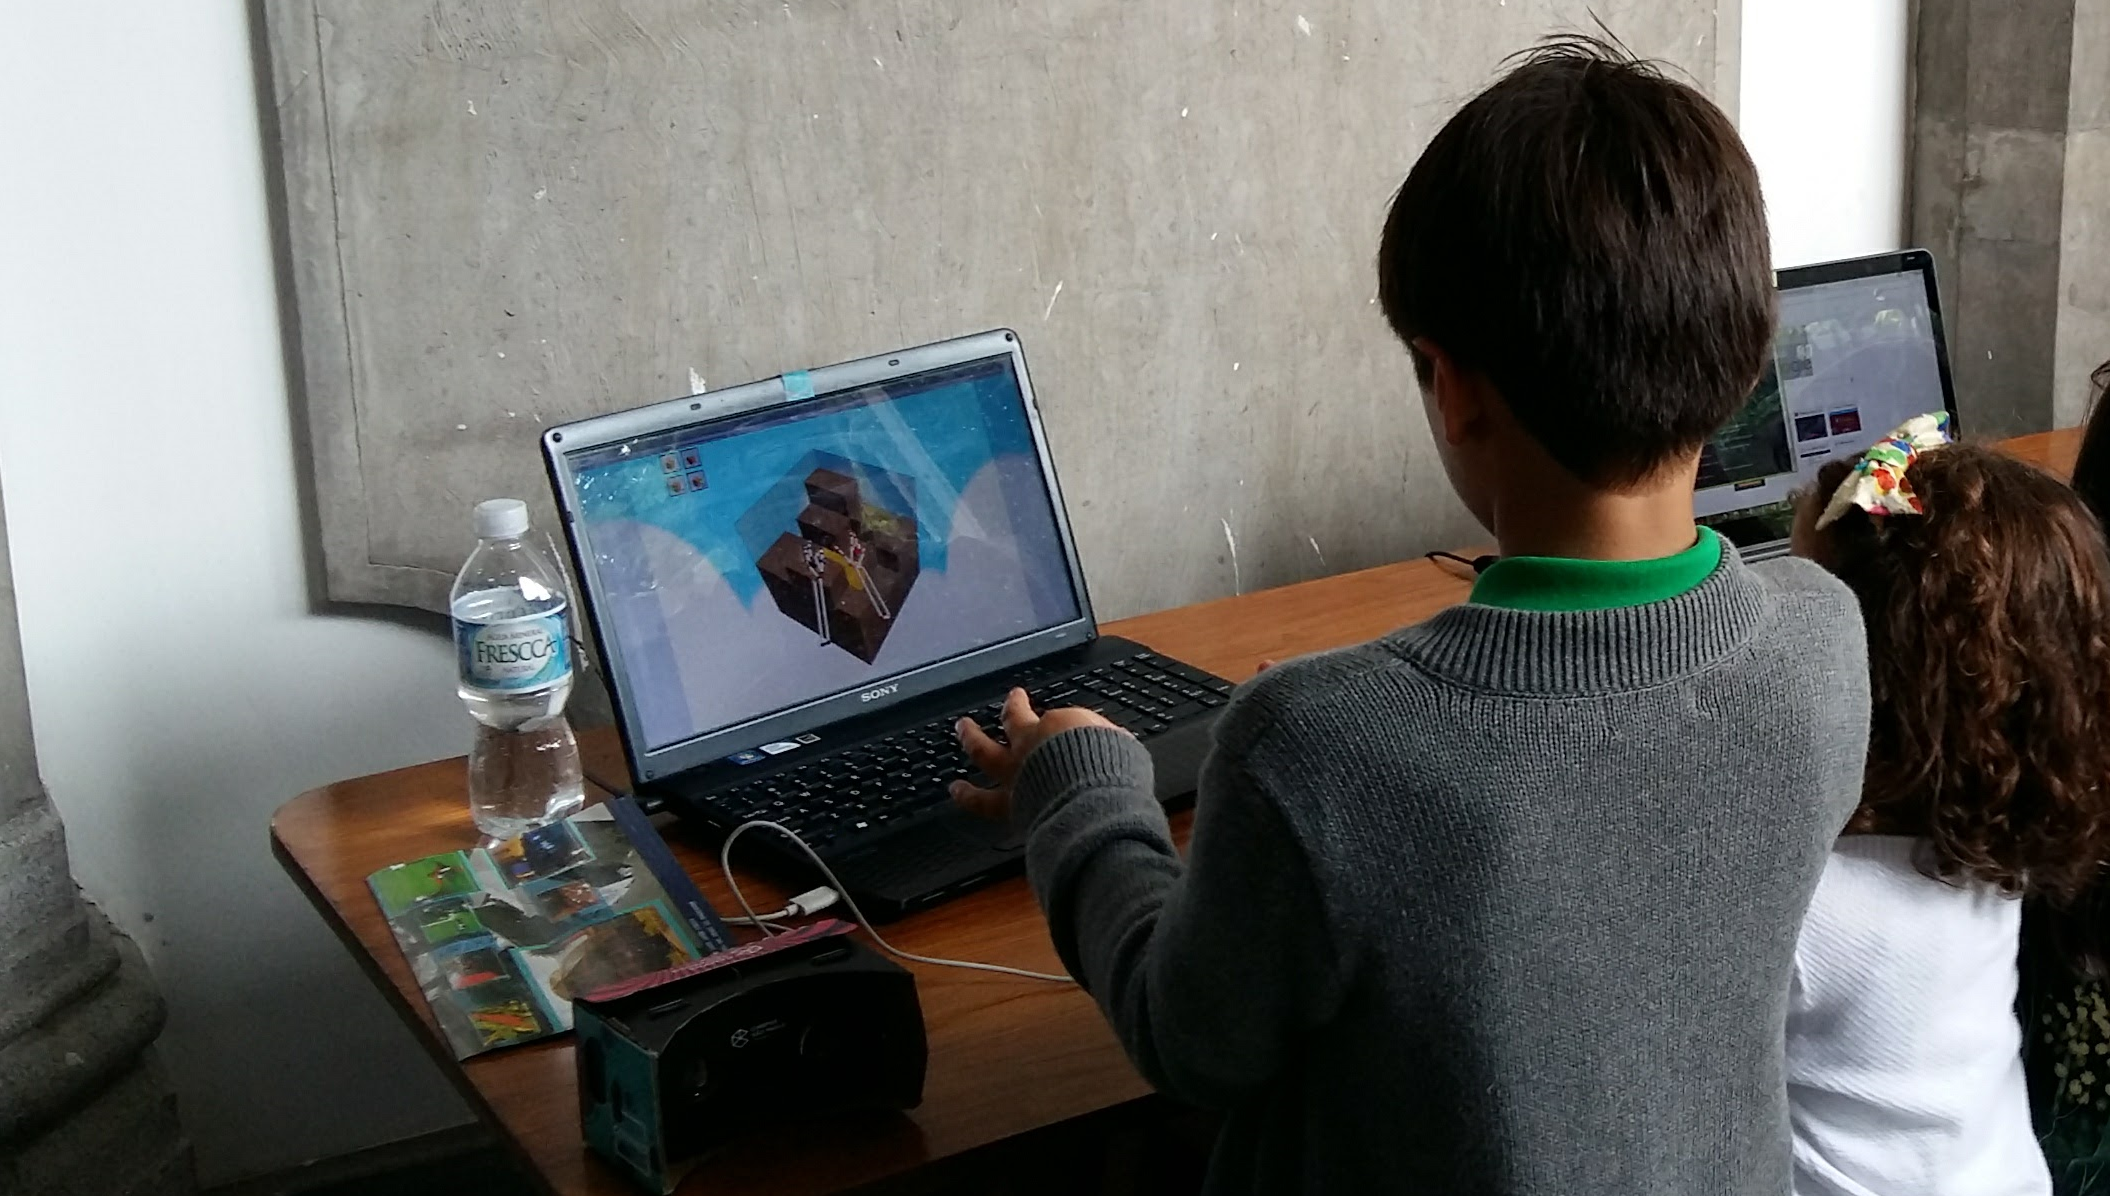
\includegraphics[width=0.5\textwidth]{tech_kids_booth2}
	\legend{\fonteAP}
	\label{fig:tech-kids-day-pc}
\end{figure}

Devido à dinâmica do evento, aonde cada bancada com algo exposto 
era visitada por várias pessoas e a rotatividade delas era alta, 
não foi possível aplicar o questionário. Mesmo assim, durante a 
execução do \textit{playtesting} 
foi notada a reação dos 
jogadores e seu \textit{feedback} foi coletado após cada sessão do jogo, 
conforme descrito na \autoref{sec-roteiro-observacoes}

\section{Observações}\label{sec-roteiro-observacoes}

Os resultados dos testes, obtidos através da observação e do 
\textit{feedback} dos jogadores, trouxeram à tona problemas inesperados, 
bem como pontos positivos na implementação escolhida.

Em termos gerais, o jogo foi bem recebido pelas crianças, que se 
mostraram entretidas e imersas durante todos os 15 minutos de sessão. Ficou claro 
também que a versão executando em realidade virtual foi mais popular, 
despertando bastante interesse nos jogadores.

Contudo, algumas interações mecânicas se revelaram mais difíceis de se 
executar do que era esperado, exigindo uma familiaridade com os sensores 
que fugia ao escopo do tempo de teste. Sobretudo as mecânicas de gerar e 
remover água se comportaram de maneira menos responsiva do que necessário 
para que o jogo pudesse ser jogado com naturalidade.

Em termos técnicos, os sensores utilizados no projeto apresentaram 
dificuldades em detectar os gestos e movimentos executados por crianças 
mais novas, devido tanto à incapacidade do \textit{Leap Motion} em 
reconhecer mãos pequenas quanto à impossibilidade das crianças em 
manter confortavelmente as mão à altura necessária para a captura 
correta de seus movimentos. 

Adicionalmente, o ambiente não colaborou com a seção de testes. A mesa 
aonde estavam dispostos os jogos se encontrava muito iluminada por 
fontes de luz, por estar do lado de uma janela. Visto que o controlador 
funciona com a captura de imagens infravermelhas, o excesso de luz 
diminuiu a qualidade de captura do controlador, interferindo no jogo.

Apesar dos desafios encontrados, a experiência geral se mostrou 
positiva, e o \textit{feedback} obtido será muito valioso para desenvolver 
iterações do projeto.

\TODO{Checar se deixamos "Será" ou "foi"}